\documentclass[13.5pt,aspecratio=169, xcolor=dvipsnames]{beamer}
\usepackage{graphicx} % Required for inserting images
\usepackage{subcaption}
\usepackage{amsfonts}
\usepackage{amsmath}
\usepackage{amssymb}
\usepackage{physics}
\usepackage{bm}
\usepackage{physics}
\usepackage{booktabs}
\usepackage{setspace}
\usepackage{xcolor}
\usepackage{wrapfig,lipsum}
\usepackage{etoolbox}
\usepackage{tikz}
\usepackage{multirow}
\usepackage{verbatim}
\usepackage{pifont}
\usepackage[most]{tcolorbox}
\usepackage{caption}
\captionsetup[figure]{labelformat=empty}%
\usetheme{Madrid}
\useinnertheme{circles}

\DeclareMathOperator*{\argmax}{arg\,max}
\DeclareMathOperator*{\argmin}{arg\,min}
\graphicspath{{Images/}{./}} 
\usetheme{Copenhagen}
\definecolor{UBCblue}{rgb}{0.04706, 0.13725, 0.26667} 
\usecolortheme[named=UBCblue]{structure}
%\usecolortheme{beaver}
% \titlegraphic{\centering \LARGE MultiVerS}
\title{An endless arcade hopper game built with \\ ThreeJs, React Native and MagicaVoxel}
\author[CS105]{
    \begin{tabular}{c}
        \textbf{CS105.O22.KHCL} \\
        \textit{Instructor: Cap Pham Dinh Thang} \\
        \bigskip
        \textbf{Group 2} \\
        Nguyen Hoang Tan \quad Pham Tram Anh \quad Le Thi Kim Yen
    \end{tabular}
}
\date{\today}
\definecolor{mylightgreencolor}{RGB}{144, 238, 144}
\definecolor{mylightredcolor}{RGB}{255, 204, 203}
\definecolor{mylightbluecolor}{RGB}{173,216,230}
\definecolor{blockbackgroundcolor}{RGB}{235,235,235}
\definecolor{blockbordercolor}{RGB}{79,79,79}

\setbeamertemplate{navigation symbols}{}
\setbeamertemplate{headline}{}
\setbeamercolor{huge text}{fg=white}
\setbeamertemplate{footline}{
    \leavevmode%
    \hbox{%
        \begin{beamercolorbox}[wd=.1\paperwidth,ht=2.25ex,dp=1ex,center]{author in head/foot}%
            \usebeamerfont{author in head/foot}\insertshortauthor
        \end{beamercolorbox}%
        \begin{beamercolorbox}[wd=.8\paperwidth,ht=2.25ex,dp=1ex,center]{title in head/foot}%
            \usebeamerfont{title in head/foot}\centering \insertshorttitle
        \end{beamercolorbox}%
        \begin{beamercolorbox}[wd=.1\paperwidth,ht=2.25ex,dp=1ex,right]{date in head/foot}%
            \insertframenumber{} / \inserttotalframenumber\hspace*{2ex} 
        \end{beamercolorbox}%
    }%
    \vskip0pt%
}
\setbeamertemplate{section in toc}{%
  \tikz[baseline=(tocseclabel.base)]{
    \node[fill=structure.fg,rounded corners,inner sep=4pt, font=\large\bfseries] (tocseclabel) {\color{white}\inserttocsectionnumber};
  }\hspace{0.5em}\large\bfseries\inserttocsection\vspace{0.3em}}


  \newtcolorbox{mybox}{
  colback=blockbackgroundcolor, % Background color (adjust as needed)
  colframe=blockbordercolor, % Frame color (adjust as needed)
  rounded corners,
  boxrule=0.2mm, % Frame width
  arc=2mm, % Radius of the rounded corners
  drop shadow, % Add a drop shadow (optional)
%   width=\tcboxwidth, % Adjust the width
%   hbox,
}




\newcommand{\raisedtext}[1]{%
  \raisebox{-0.2ex}{#1}%
}
  
\begin{document}
\begin{frame}
    \begin{picture}(0,0)
        \put(170,0){\makebox(0,0){\huge \textbf{\textcolor{UBCblue}{Crossy Road}}}}
    \end{picture}
    \maketitle
\end{frame}

% \begin{frame}
% 	\frametitle{Table of Contents} % Slide title, remove this command for no title
% 	\tableofcontents[subsectionstyle=hide]
% \end{frame}
%-------------------------------------------------------------------%


% \begin{frame}
%     \doublespacing
%         \frametitle{Presentation Overview} % Slide title, remove this command for no title
        
%         \tableofcontents % Output the table of contents (all sections on one slide)
%         %\tableofcontents[pausesections] % Output the table of contents (break sections up across separate slides)
% \end{frame}
    
%     %----------------------------------------------------------------------------------------
%     %	PRESENTATION BODY SLIDES
%     %----------------------------------------------------------------------------------------
    
%     \section{Lexical Semantics} % Sections are added in order to organize your presentation into discrete blocks, all sections and subsections are automatically output to the table of contents as an overview of the talk but NOT output in the presentation as separate slides
%     %------------------------------------------------
%     \begin{frame}
%         \doublespacing
%             \frametitle{Presentation Overview} % Slide title, remove this command for no title
            
%             \tableofcontents[currentsection] % Output the table of contents (all sections on one slide)
%             %\tableofcontents[pausesections] % Output the table of contents (break sections up across separate slides)
%     \end{frame}

% %-------------------------------------------------------------------%

\begin{frame}
    \onehalfspacing
    \frametitle{Voxel Art}
    \textbf{What are voxels:}
    \vspace*{-1em} 
    \begin{mybox}
        A voxel is a cube, also known as a 3D pixel \\
        The word voxel is derived form the words “volumetric pixel”
      \end{mybox}

      \centering
      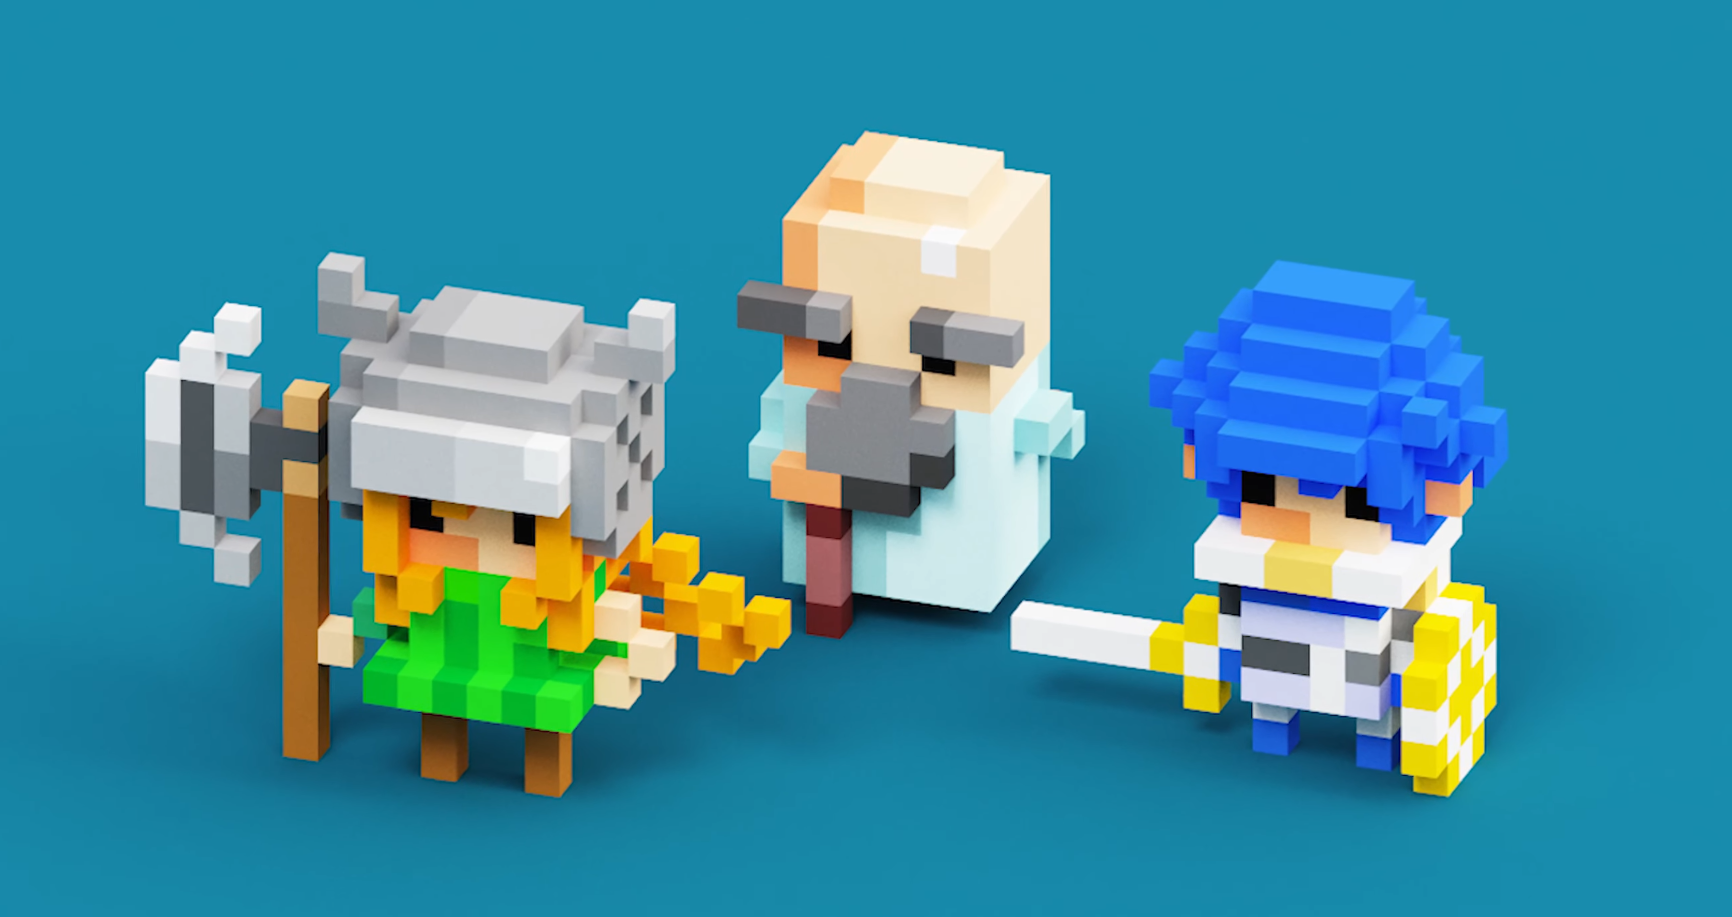
\includegraphics[scale=0.15]{Voxel_Art_Example.png}
\end{frame}
    
%--------------------------------------------------



\begin{frame}
    \onehalfspacing
    \frametitle{MagicaVoxel}
    \begin{minipage}{0.5\textwidth}
            \begin{block}{}
                A free lightweight 8-bit voxel editor 
            \end{block}

            \vspace{0.5em}
            \centering
            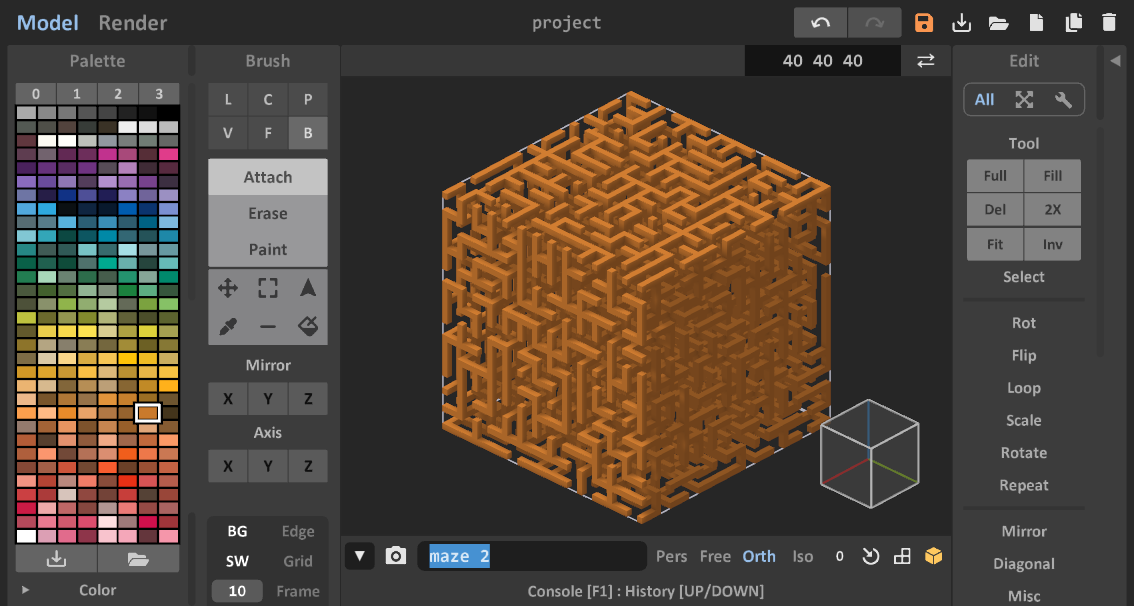
\includegraphics[width=\textwidth]{magica_commands.png}
    \end{minipage}
    \begin{minipage}{0.49\textwidth}
        \centering
        
\includegraphics[height=0.85\textheight]{CS_er_model.png}
\end{minipage}
\end{frame}
    
%--------------------------------------------------

    \begin{frame}
    \onehalfspacing
        \frametitle{Crossy Road}
        \begin{mybox}
        Players control a character to survive an endless series of obstacles
        \end{mybox}
        \centering
        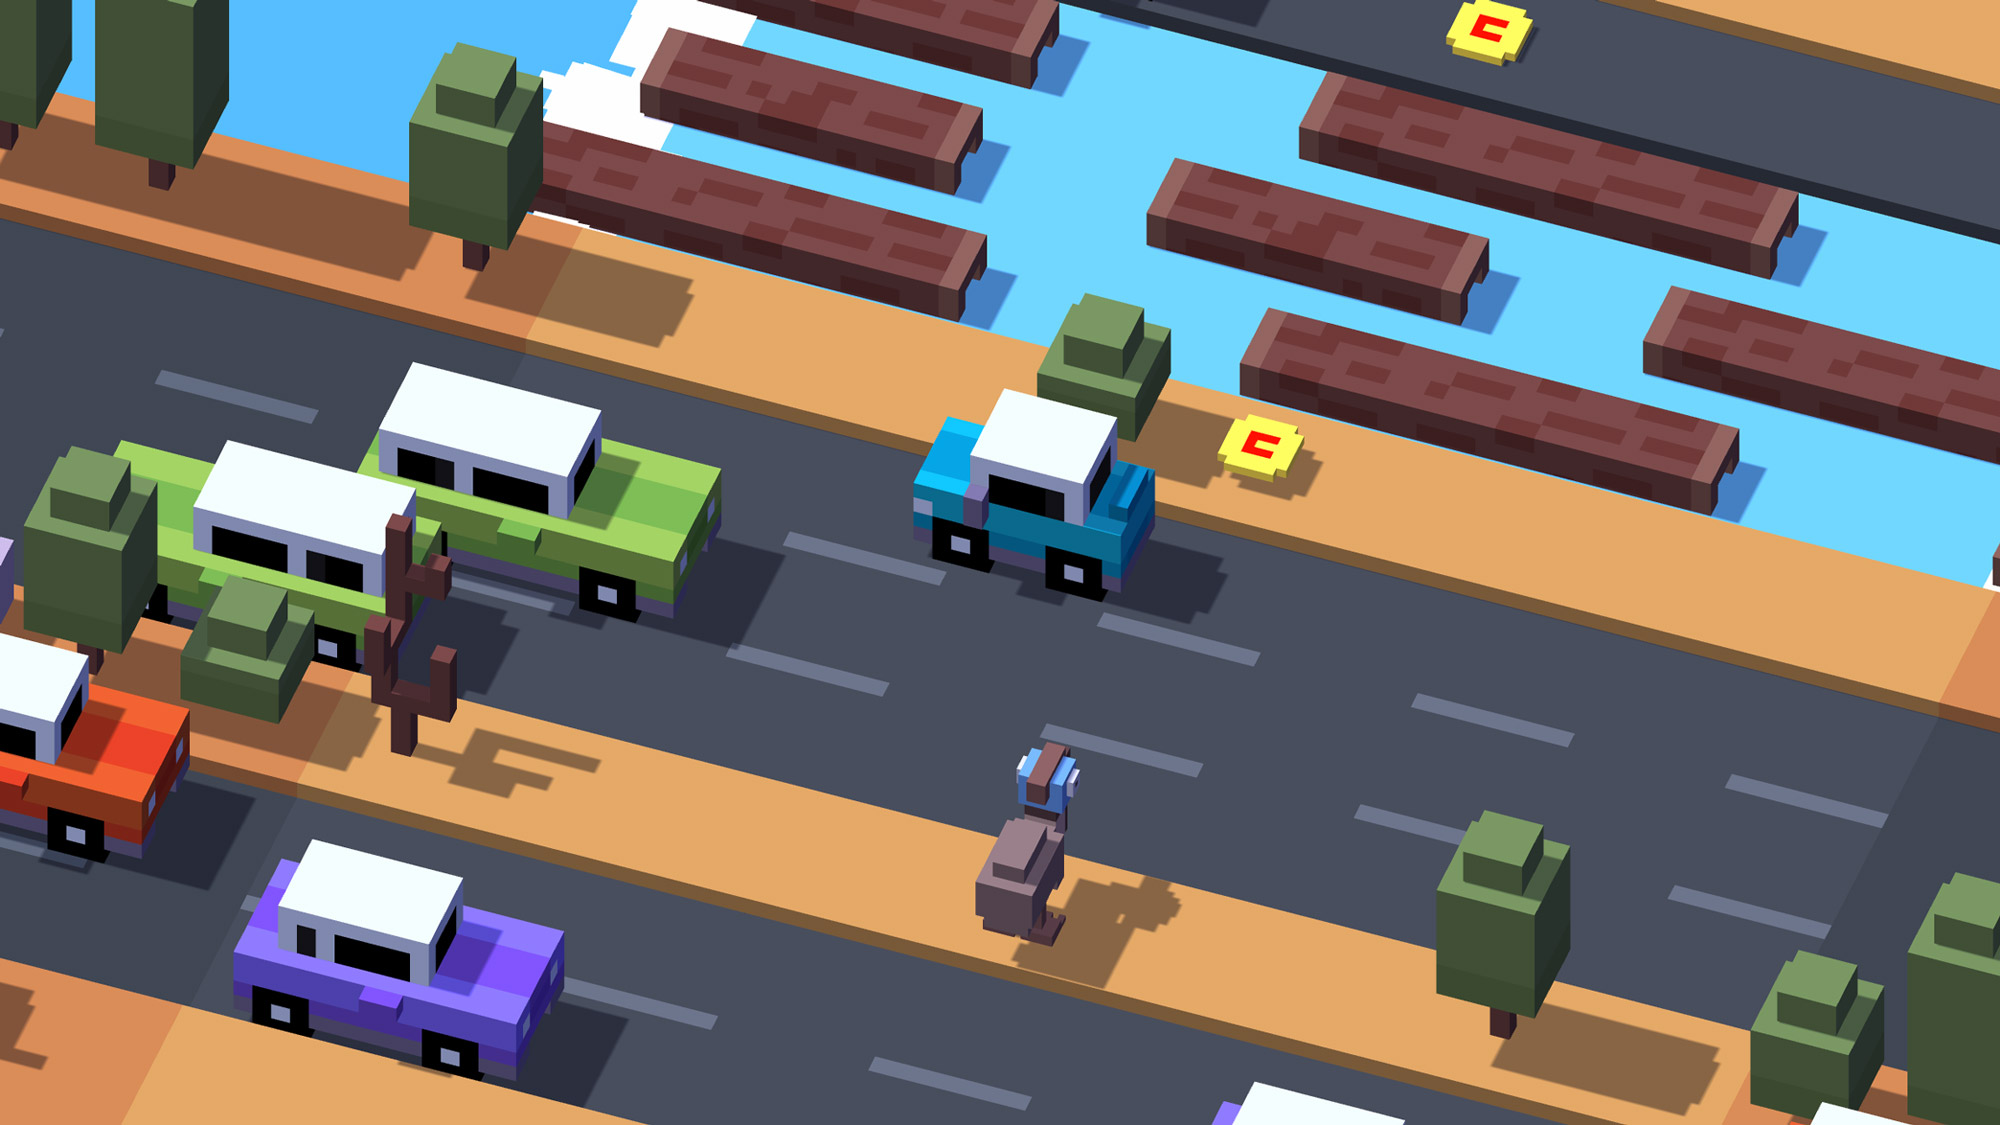
\includegraphics[width=0.9\textwidth]{crossy_road.jpg}
    \end{frame}
    
    
    %------------------------------------------------

    \begin{frame}
        \onehalfspacing
        \frametitle{Tech Stack}

        \begin{figure}[h]
            \begin{minipage}{0.32\textwidth}
                \centering
                {
\includegraphics[height=0.4\textheight]{Icons/react_native_web.png}}
                \caption{React Native Web}
            \end{minipage}
            \begin{minipage}{0.32\textwidth}
                \centering
                
\includegraphics[height=0.4\textheight]{Icons/MagicaVoxel.png}
                \caption{MagicaVoxel}
            \end{minipage}
            \begin{minipage}{0.32\textwidth}
                \centering
                
\includegraphics[height=0.4\textheight]{Icons/three-js-logo-07A32307F1-seeklogo.com.png}
                \caption{Three.js}
            \end{minipage}
        \end{figure}

       
    
    \end{frame}
        
    %--------------------------------------------------
    
    \begin{frame}
        \onehalfspacing
        \frametitle{Tasks to Complete}
        \only<1> {
            \begin{minipage}{0.25\textwidth}
                \begin{block}{}
                    \centering
                    Time System
                \end{block}
            \end{minipage}
    
            \begin{figure}[h]
                \begin{minipage}{0.4\textwidth}
                    \centering
                    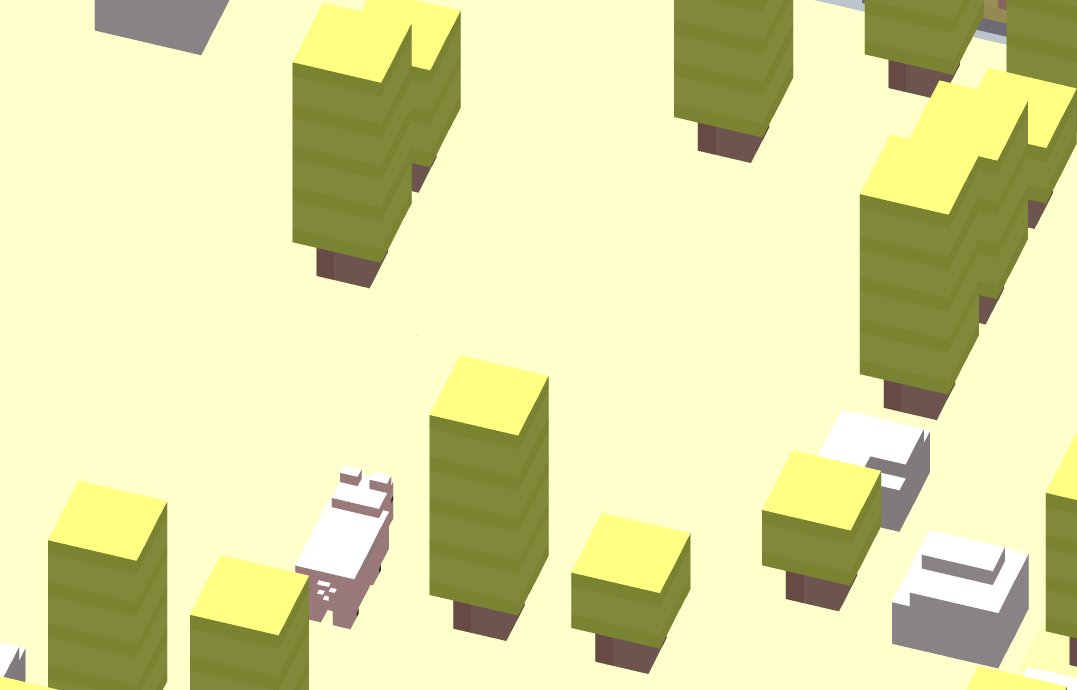
\includegraphics[height=0.4\textheight, width=\textwidth]{time_system_day.png}
                    \caption{Day}
                \end{minipage}
                \begin{minipage}{0.5\textwidth}
                    \centering
                    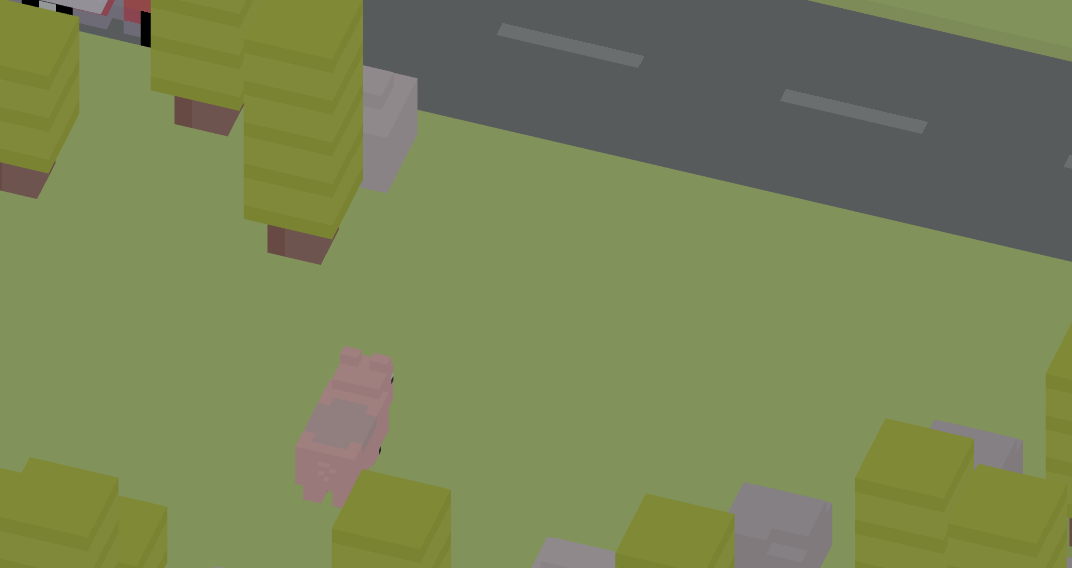
\includegraphics[height=0.4\textheight, width=0.85\textwidth]{time_system_night.png}
                    \caption{Night}
                \end{minipage}
            \end{figure}
        }
    
    
        \only<2> {
            \begin{minipage}{0.4\textwidth}
                \begin{block}{}
                    \centering
                    Dynamic Shadow Effect
                \end{block}
            \end{minipage}
    
            \begin{figure}[h]
                \begin{minipage}{0.4\textwidth}
                    \centering
                    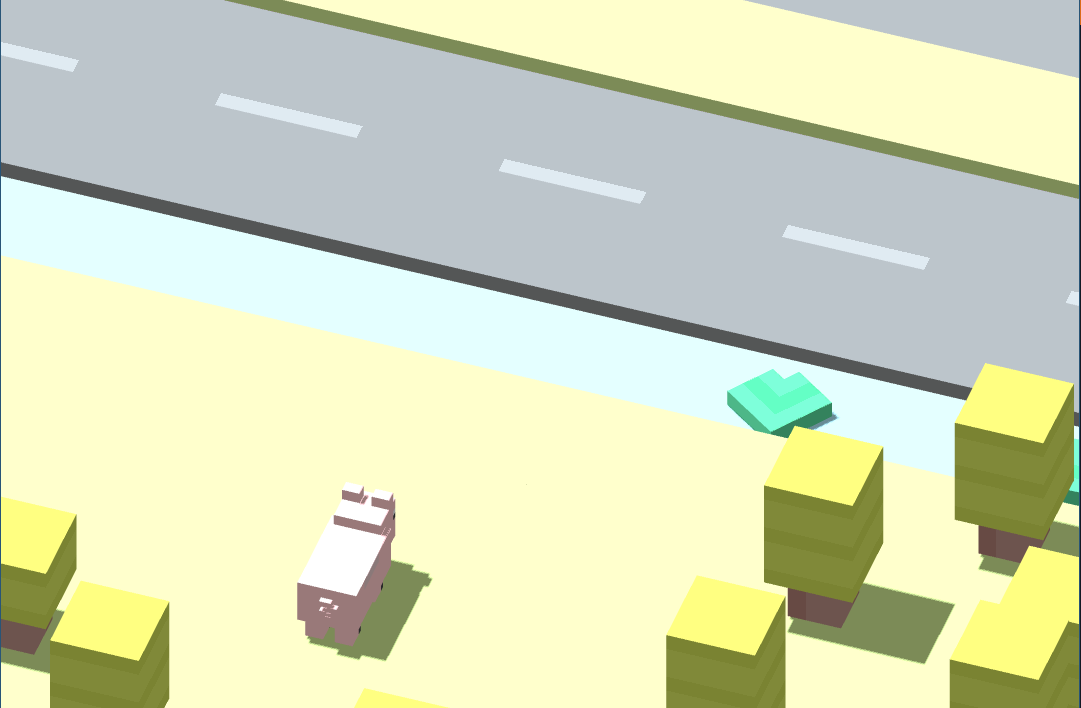
\includegraphics[height=0.4\textheight, width=1.1\textwidth]{shadow_right.png}
                    \caption{Day}
                \end{minipage}
                \begin{minipage}{0.5\textwidth}
                    \centering
                    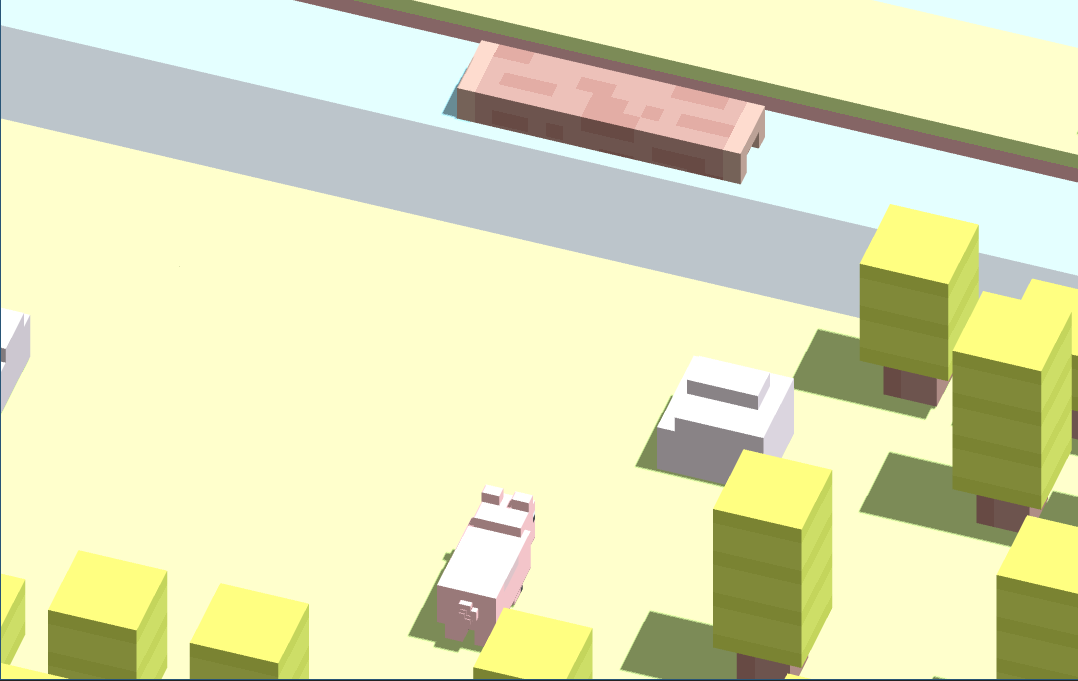
\includegraphics[height=0.4\textheight, width=0.85\textwidth]{shadow_left.png}
                    \caption{Night}
                \end{minipage}
            \end{figure}
        }
    
    
        \only<3> {
            \begin{minipage}{0.4\textwidth}
                \begin{block}{}
                    \centering
                    Additional Themes \& Items
                \end{block}
            \end{minipage}
    
            \begin{figure}[h]
                \centering
                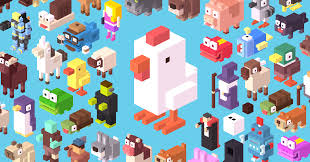
\includegraphics[width=0.8\textwidth]{multi_theme.jpg}
            \end{figure}
        }
    
        \only<4> {
            \begin{minipage}{0.4\textwidth}
                \begin{block}{}
                    \centering
                    Multiplayer Functionality
                \end{block}
            \end{minipage}
    
            \begin{figure}[h]
                \centering
                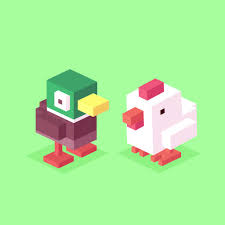
\includegraphics[width=0.5\textwidth]{Multiplayer.jpg}
            \end{figure}
        }
    \end{frame}
    
    \begin{frame}
        \begin{center}
            {\Huge Thank you for your attention!}
            
            \bigskip\bigskip % Vertical whitespace
            
            {\LARGE Feedback Section}
        \end{center}
    \end{frame}
    


\end{document}
